%%%%%%%%%%%%%%%%%%%%%%%%%%%%%%%%%%%%%%%
% a0poster Landscape Poster
% LaTeX Template
% Version 1.0 (22/06/13)
%
% The a0poster class was created by:
% Gerlinde Kettl and Matthias Weiser (tex@kettl.de)
% 
% This template has been downloaded from:
% http://www.LaTeXTemplates.com
%
% License:
% CC BY-NC-SA 3.0 (http://creativecommons.org/licenses/by-nc-sa/3.0/)
%
%%%%%%%%%%%%%%%%%%%%%%%%%%%%%%%%%%%%%%%%%

%----------------------------------------------------------------------------------------
%	PACKAGES AND OTHER DOCUMENT CONFIGURATIONS
%----------------------------------------------------------------------------------------

% aspb is 3'7'' x 3'6''
\documentclass[aspb,landscape]{a0poster}

\usepackage{fontspec}
\usepackage[svgnames]{xcolor} % enable specifying colors by their 'svgnames', for a full list of all colors available see here: http://www.latextemplates.com/svgnames-colors

% Carnegie uses Roboto Slab (serif) and Lato (sans serif)
\setmainfont[Ligatures=TeX]{Lato}

% Carnegie colors
\definecolor{CarnegiePriBlue}{cmyk}{1.00,0.85,0.15,0.25}  % main primary blue
\definecolor{CarnegieSecBlue1}{cmyk}{0.68,0.48,0.00,0.00} % first secondary blue
\definecolor{CarnegieSecBlue2}{cmyk}{0.85,0.69,0.04,0.00} % second secondary blue

\definecolor{CarnegiePriTurq}{cmyk}{0.60,0.10,0.15,0.00}  % main primary turquoise

\definecolor{CarnegiePriGreen}{cmyk}{0.46,0.00,0.90,0.00} % main primary green

\definecolor{CarnegiePriBrown}{cmyk}{0.25,0.40,0.65,0.00} % main primary brown

% multiple columns
\usepackage{multicol} % This is so we can have multiple columns of text side-by-side
\columnsep=100pt      % This is the amount of white space between the columns in the poster
\columnseprule=3pt    % This is the thickness of the black line between the columns in the poster
\def\columnseprulecolor{\color{lightgray}}

% other needed packages
\usepackage{amsfonts, amsmath, amsthm, amssymb} % For math fonts, symbols and environments
\usepackage{wrapfig}  % Allows wrapping text around tables and figures
\usepackage{graphicx} % Required for including images
\usepackage{booktabs} % Top and bottom rules for table

% tweak figure and table captions
\usepackage[font=small,labelfont={bf,color=CarnegiePriBlue},textfont={color=CarnegiePriBlue},margin=0pt,skip=18pt]{caption}

% natbib drops numbers and we'll shrink text size; drop labels
\usepackage{natbib}
\def\bibfont{\footnotesize}
\makeatletter
\renewcommand\@biblabel[1]{}
\makeatother

% tweak list spacing
\usepackage{enumitem}
\setlist[itemize]{topsep=10pt,itemsep=8pt,itemindent=48pt}
\setlist[enumerate]{topsep=10pt,itemsep=8pt,itemindent=48pt}

% tweak paragraphs
\setlength{\parindent}{0pt}
\setlength{\parskip}{12pt}

% tweak title spacing and colors
% \titlespacing{command}{left spacing}{before spacing}{after spacing}[right]
% spacing: how to read {12pt plus 4pt minus 2pt}
%          12pt is what we would like the spacing to be
%          plus 4pt means that TeX can stretch it by at most 4pt
%          minus 2pt means that TeX can shrink it by at most 2pt
\usepackage{titlesec}
\titlespacing{\section}{0pt}{24pt}{0pt}
\titlespacing{\subsection}{0pt}{1em}{1em}
\titlespacing{\subsubsection}{0pt}{12pt}{0pt}
\titleformat{\section}{\color{CarnegiePriBlue}\Large\bfseries}{\color{CarnegiePriBlue}\thesection}{1em}{}
\titleformat{\subsection}{\color{CarnegieSecBlue1}\large\bfseries}{\color{CarnegieSecBlue1}\thesubsection}{1em}{}

% tweak equation whitespace
%% \abovedisplayskip=12pt plus 3pt minus 9pt
%% \abovedisplayshortskip=0pt plus 3pt
%% \belowdisplayskip=12pt plus 3pt minus 9pt
%% \belowdisplayshortskip=7pt plus 3pt minus 4pt

% width of figures for consistency
\newlength{\figwidth}
\setlength{\figwidth}{320mm}

% space above figures
\newlength{\figtopspace}
\setlength{\figtopspace}{18pt}

\graphicspath{{figures/}} % Location of the graphics files

\begin{document}

%----------------------------------------------------------------------------------------
%	POSTER HEADER 
%----------------------------------------------------------------------------------------

% The header is divided into three boxes:
% The first is 55% wide and houses the title, subtitle, names and university/organization
% The second is 25% wide and houses contact information
% The third is 19% wide and houses a logo for your university/organization or a photo of you
% The widths of these boxes can be easily edited to accommodate your content as you see fit
% Note: no line breaks between minipage environments!

{
  \color{CarnegiePriBlue} \VeryHuge
  \textbf{Model-Based Quantification of Induced Gene Expression Time Courses}    % Title
}
\vspace{5mm}

\begin{minipage}[m]{0.08\linewidth}
  
\includegraphics[height=70mm]{sam-bfr-smiling-crop.jpg} % author photo
\end{minipage}
\begin{minipage}[m]{0.40\linewidth}                      % Author(s)
  \color{Black}
  \Huge \textbf{Sam Hokin \& M. Kathryn Barton} \\
  \Large shokin@carnegiescience.edu
\end{minipage}
\begin{minipage}[m]{0.49\linewidth}
  
\includegraphics[height=70mm]{CS_plantbio_logo_horz.eps} % Carnegie DPB logo
\end{minipage}

\vspace{10mm} % A bit of extra whitespace between the header and poster content
\color{CarnegiePriBlue}
\hrulefill

\color{Black}

%% \color{DarkSlateGray}\Large \textbf{Contact Information:}\\
%% Department Name\\ % Address
%% University Name\\
%% 123 Broadway, State, Country\\\\
%% Phone: +1 (000) 111 1111\\ % Phone number
%% Email: \texttt{john@LaTeXTemplates.com}\\ % Email address


%----------------------------------------------------------------------------------------

\begin{multicols}{3} % This is how many columns your poster will be broken into, a poster with many figures may benefit from less columns whereas a text-heavy poster benefits from more

  \color{Black} % default color

  %----------------------------------------------------------------------------------------
  %	ABSTRACT
  %----------------------------------------------------------------------------------------

  %% \begin{abstract}
  %% \end{abstract}

  %----------------------------------------------------------------------------------------
  %	INTRODUCTION
  %----------------------------------------------------------------------------------------

  {
    \titlespacing{\section}{0pt}{0pt}{0pt}
    \section*{INTRODUCTION}

    \textbf{We model gene expression time courses following induction of a glucocorticoid receptor-bound transcription factor into the nucleus after exposure to dexamethasone in Arabidopsis thaliana.}
    
    In contrast to single-time measurements of induced expression, which result in a single fold-change value, typically long after the induction event,
    our model reproduces the dynamics of TF import into the nucleus followed by the transcriptional dynamics of its direct and indirect targets.
    
    \textbf{The model quantifies an observed time course with two rate coefficients}:
    \begin{enumerate}
    \item $\hat{\eta}_p$ = the normalized initial rate of rise (+) or fall (-) of target mRNA levels
    \item $\gamma_p$ = the mRNA loss rate
    \end{enumerate}
    \textbf{These two processes compete to determine the final transcript fold change:} a highly-induced transcript may saturate at a low fold change if it also decays quickly,
    while weakly-induced transcripts may rise to a high level if they have very low loss.
    
    \textbf{In addition, some targets exhibit ``turn-off'', or auto-regulation}. These time courses require a turn-off time, $t_{off}$, after which the mRNA level decays exponentially at $\gamma_p$.
    
    We present analysis of experiments with GR-TFs involved in leaf regulation:
    \begin{itemize}
    \item GR-STM: AT1G62360 \textit{SHOOT MERISTEMLESS/STM}
    \item GR-AS2: AT1G65620 \textit{ASYMMETRIC LEAVES 2/AS2/LBD6}
    \item GR-KAN: AT5G16560 \textit{KANADI 1/KAN1}
    \item GR-TINY: AT5G25810 \textit{TINY}
    \item GR-REV: AT5G60690 \textit{REVOLUTA/REV}
    \end{itemize}
    
    Our experiments measure expression time courses for up to two hours after DEX exposure with both RNA-seq and microarray assays.
    Since secondary targets of the induced transcription factor are expected to rise after some delay, during which the primary transcript's protein level rises,
    we explore the use of our model to distinguish between primary and secondary targets.

  }

  %----------------------------------------------------------------------------------------
  %	OBJECTIVES
  %----------------------------------------------------------------------------------------

  \section*{OBJECTIVES}
  \color{CarnegiePriBlue}  

  {
    \setlist[enumerate]{itemindent=0pt}
    \begin{enumerate}
    \item Model the import of the GR-TF into the nucleus after DEX exposure
    \item Model the modified transcription of GR-TF primary targets (subscript $p$)
    \item Model the modified transcription of GR-TF secondary targets (subscript $s$), which are primary targets of GR-TF primary targets
    \item Compare the model-fitted rate coefficients with standard fold-change analysis
    \end{enumerate}
  }

  \color{Black}

  %----------------------------------------------------------------------------------------
  %	MATERIALS AND METHODS
  %----------------------------------------------------------------------------------------

  \section*{MODEL AND EXPERIMENTAL METHOD}

  %% Could have introductory text here before subsections.

  %------------------------------------------------

  \subsection*{Nuclear import model}

  Transport of a glucocorticoid receptor (GR) into the nucleus after DEX application has been measured in animal tissue by several groups.

  \begin{center}\vspace{\figtopspace}
    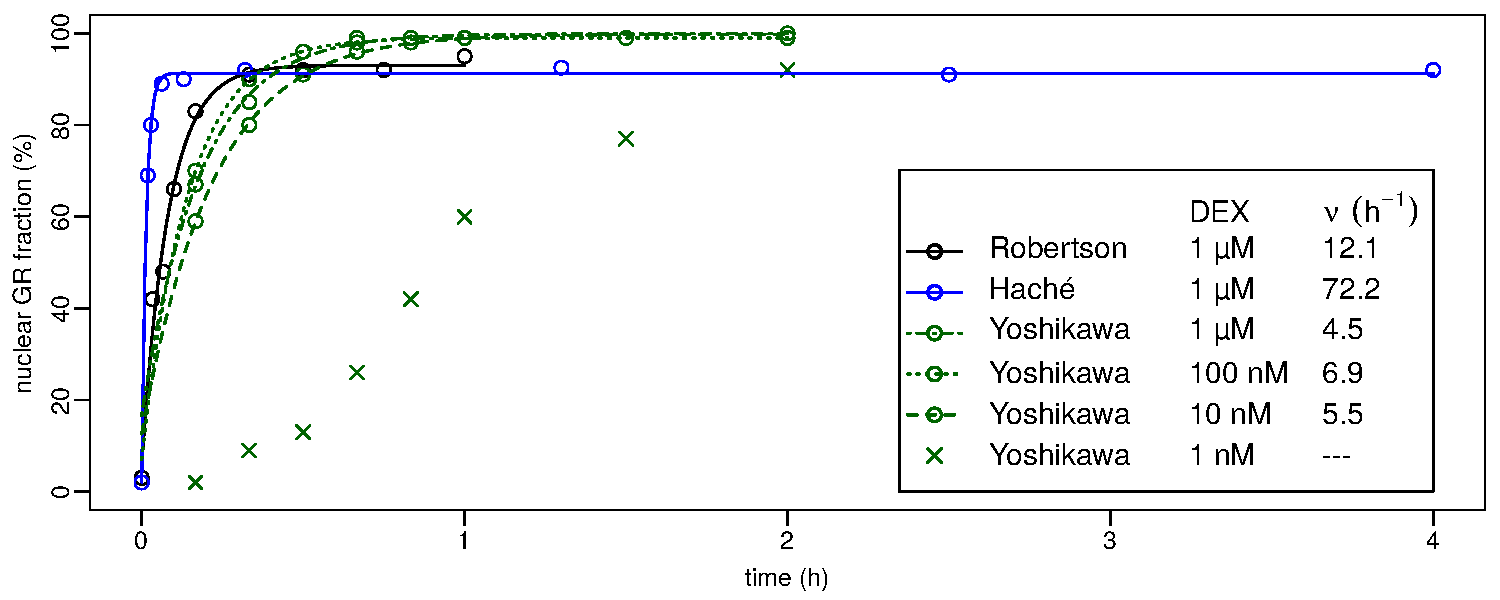
\includegraphics[width=\figwidth]{robertson-hache-yoshikawa}
    \captionof{figure}{
      The measured nuclear GR concentration follows a saturated exponential time course, except at very low DEX concentration. Data sources in References.
    }
  \end{center}
  
  The measured time courses are well described by a pair of linear ODEs:
  \begin{eqnarray*}\label{eq:rho_c_de}
    \dot{\rho_c} &=& -\nu \rho_c + \gamma_e \rho_n \\
    \dot{\rho_n} &=&  \nu \rho_c - \gamma_e \rho_n - \gamma_n \rho_n
  \end{eqnarray*}
  \begin{eqnarray*}
    \rho_c &=& \text{cytoplasmic GR protein concentration} \\
    \rho_n &=& \text{nuclear GR protein concentration} \\
    \nu &=& \text{nuclear import rate} \\
    \gamma_e &=& \text{nuclear export rate} \\
    \gamma_n &=& \text{rate of loss of GR-TF from other causes}
  \end{eqnarray*}
  We neglect nuclear export and loss setting $\gamma_e=0$ and $\gamma_n=0$ since those rates are slow compared to our two-hour measurement span.
  We assume that import of chimeric GR-TF is similar to the published GR import data.

  \subsection*{Transcription model}

  We model altered transcription of target mRNA due to DEX-induced import of the GR-TF with a set of coupled ODEs:
  \begin{eqnarray*}
    \dot{\rho_p} &=& \eta_p \rho_n  - \gamma_p \rho_p  \\
    \dot{\rho_s} &=& \eta_s \rho_p  - \gamma_s \rho_s 
  \end{eqnarray*}
  \begin{eqnarray*}
    \rho_p &=& \text{expressed mRNA/protein of a primary target of the GR-TF} \\
    \rho_s &=& \text{expressed mRNA/protein of a secondary target of the GR-TF, i.e. target of a primary target} \\
    \gamma_p &=& \text{loss rate of primary mRNA/protein} \\
    \gamma_s &=& \text{loss rate of secondary mRNA/protein} \\
    \eta_p &=& \text{transcription rate between the GR-TF and primary target} \\
    \eta_s &=& \text{transcription rate between the primary and secondary targets}
  \end{eqnarray*}
  We assume that mRNA and protein concentrations are in fixed proportion, so that $\rho_p$ and $\rho_s$ represent measured mRNA levels as well as protein concentration.
  (This avoids two more equations and four more fit parameters accounting for translation.)
  $\gamma_p$ and  $\gamma_s$ represent loss of mRNA.

  These equations can be solved analytically, and set $\nu=10 {\rm h}^{-1}$ based on the animal tissue studies (we need to measure it!).
  
  \subsection*{Primary target expression time course metrics}

  The model provides two useful, independent time course  metrics:
  \begin{itemize}
    \item $\hat{\eta}_p  = \eta_p \rho_n(0) / \rho_p(0)$ characterizes the initial change of mRNA level
    \item $\gamma_p$ characterizes the loss of mRNA
  \end{itemize}
  In addition, we can calculate an asymptotic ($t\rightarrow\infty$) fold change:
  \begin{equation*}
    {\rm logFC}_\infty \equiv \lim_{t \to \infty} \log_2\frac{\rho_p(t)}{\rho_p(0)} = \log_2\left(1 + \frac{\hat{\eta}_p}{\gamma_p} \frac{\rho_c(0)}{\rho_n(0)} \right)
  \end{equation*}
  The ratio $\hat{\eta_p}/\gamma_p$ therefore determines the asymptotic fold change of a transcript: \textbf{mRNA transcription and loss play equal roles in the final transcript level in this model}.

  \subsection*{Time-course expression measurements in {\it Arabidopsis thaliana}}

  The five GR-TF plant lines plus WT plants (all Col-0) were grown to seedlings, and tissue was exposed to 50 $\mu$M of DEX and then flash frozen 0, 0.5, 1 and 2 hours later.
  Almost all samples had at least three biological replicates per time. RNA was extracted and assayed with the Affymetrix ATH1 microarray and Illumina HiSeq RNA-seq.
  The microarray data were analyzed using the R packages \texttt{affy} and \texttt{limma}; the RNA-seq data were analyzed using TopHat2, Cufflinks and Cuffdiff.
  Sequences were mapped to the TAIR10 reference genome. 

  %----------------------------------------------------------------------------------------
  %	RESULTS 
  %----------------------------------------------------------------------------------------

  \section*{RESULTS}

  \subsection*{Expression time courses exhibit qualitative variation}

  \textbf{It matters greatly \underline{when} you measure differential expression in an induced expression experiment!}
  
  \begin{center}\vspace{\figtopspace}
    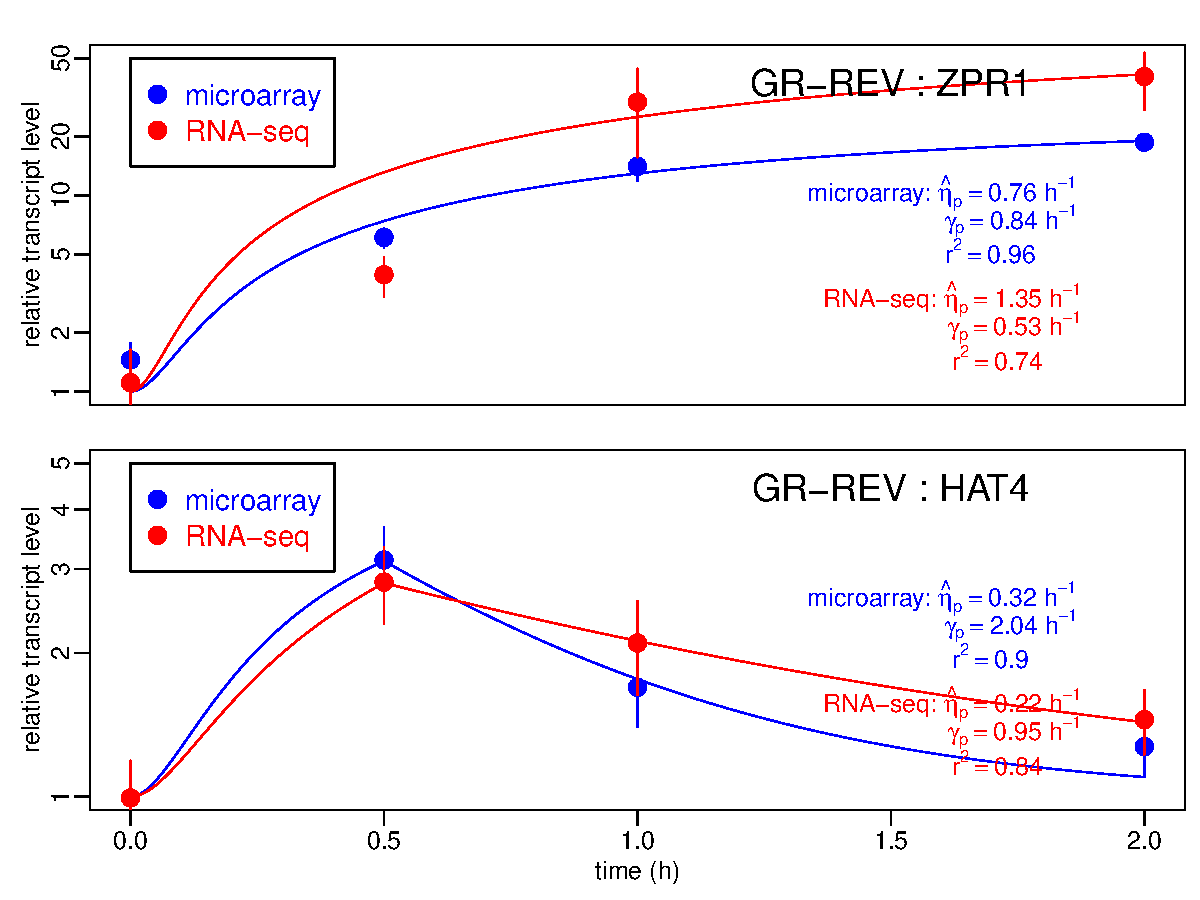
\includegraphics[width=\figwidth]{ZPR1-HAT4}
    \captionof{figure}{
      Expression time courses vary greatly, from strong GR-REV monotonic risers like \textit{ZPR1} to HD-ZIPII self-regulators like \textit{HAT4}. Lines represent primary target model fits
      with transcription turned off at $t=0.5$ h for \textit{HAT4}.
    }
  \end{center}

  \subsection*{Model parameters $\hat{\eta}_p$ and $\gamma_p$ distinguish expression time course shapes}
  
  \begin{center}\vspace{\figtopspace}
    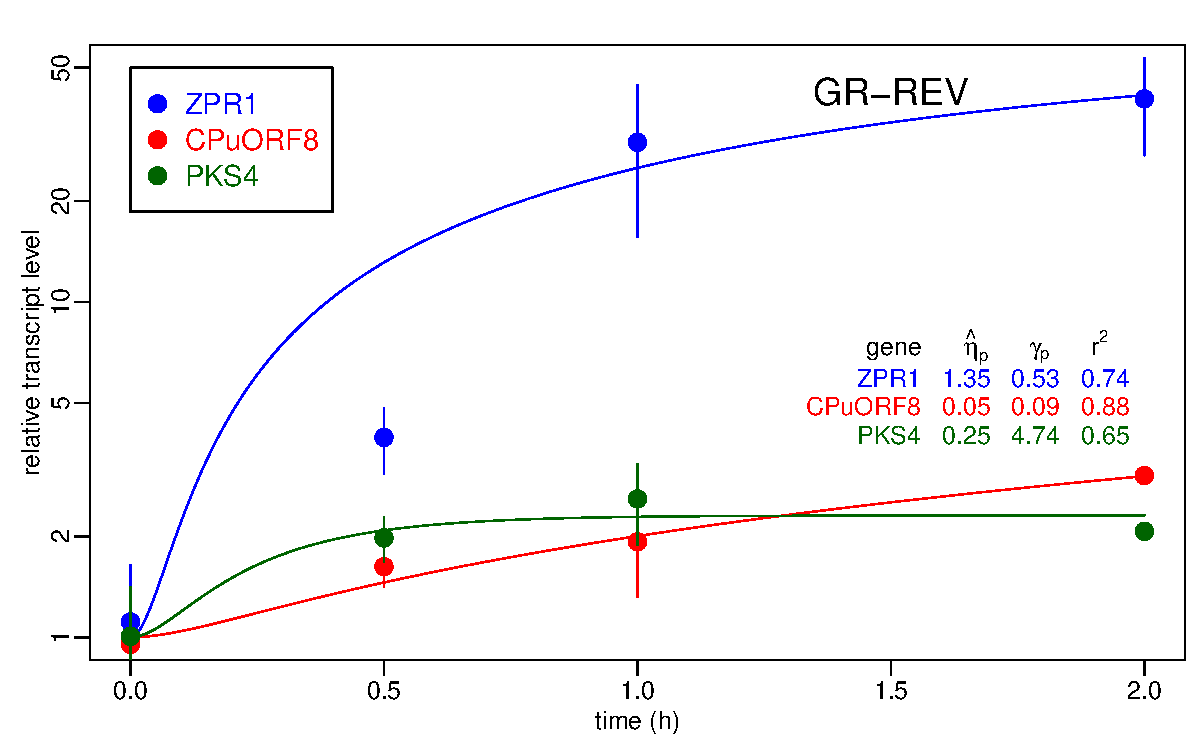
\includegraphics[width=\figwidth]{ZPR1-CPuORF8-PKS4}
    \captionof{figure}{
      Three distinct time course shapes result from:
      high $\hat{\eta}_p$ and low $\gamma_p$ for \textit{ZPR1}, the most strongly regulated GR-REV target; 
      low $\hat{\eta}_p$ and low $\gamma_p$ for \textit{CPuORF8}, which reaches a significant fold-change due to low loss;
      and high $\hat{\eta}_p$ and high $\gamma_p$ for \textit{PKS4}, which saturates quickly due to high loss.
    }
  \end{center}

  Three examples that exhibit very different transcriptional responses to DEX application:
  \begin{itemize}
  \item \textit{ZPR1} is the most strongly up-regulated target of GR-REV --- a strong, steady riser with a strong initial transition ($\kappa$ is large) leading to a large asymptotic DE level (${\rm logFC}_\infty$ is large).
  \item \textit{CRK30} is the most strongly down-regulated target of GR-KAN in the RNA-seq series --- it is predicted to reach a larger DE level further out in time.
  \item \textit{HAT22} is a strong autoregulating GR-REV target --- an early rise with a large $\kappa$ value is followed by ``turn-off'' after $t=0.5$ h; without turn-off, the model predicts it would reach $\rm logFC_\infty=1.8$.
  \end{itemize}

  \begin{center}
    \begin{tabular}{c|ccc|cc}
      \multicolumn{1}{c}{}        & \multicolumn{3}{c}{logFC} & \multicolumn{2}{c}{model} \\ 
      \multicolumn{1}{c}{gene (assay)} & 0.5h & 1.0h & \multicolumn{1}{c}{2.0h}  & $\kappa$        & $\rm logFC_\infty$ \\
      \midrule
      \textit{ZPR1}  (microarray) & 2.09 & 3.29 & 3.71         & 122 $\rm h^{-2}$ & 4.06 \\
      \textit{CRK30} (RNA-seq)    & -0.72 & -1.93 & -2.51      & -15 $\rm h^{-2}$ & -3.01 \\
      \textit{HAT22} (microarray) & 1.53 & $\times$ & $\times$ &  96 $\rm h^{-2}$ & 1.77 \\
    \end{tabular}
    \captionof{table}{
      \texttt{limma} and Cuffdiff DE levels along with model-derived metrics $\kappa$ and $\rm logFC_\infty$.
    }
  \end{center}

  Intermediate DE values, given by logFC, depend on the time of measurement while $\kappa$ and ${\rm logFC}_\infty$ characterize the entire time course.

  \subsection*{Early-peaking primary transcripts are well fit by mid-course transcription turn-off in the model}

  When $\gamma_n=0$, only group L time courses can be fit by the model with constant $\eta_p$. Group E and M genes appear to exhibit transcription
  ``turn-off'' --- after a certain amount of time (or beyond a certain level of expression) transcription of those genes' mRNA ``turns off'' and the subsequent transcript level
  drops as $e^{-\gamma_p t}$. We model transcription turn-off by setting $\eta_p=0$ at $t=0.5$h for E time courses and $t=1.0$h for M time courses.

  \begin{center}\vspace{\figtopspace}
    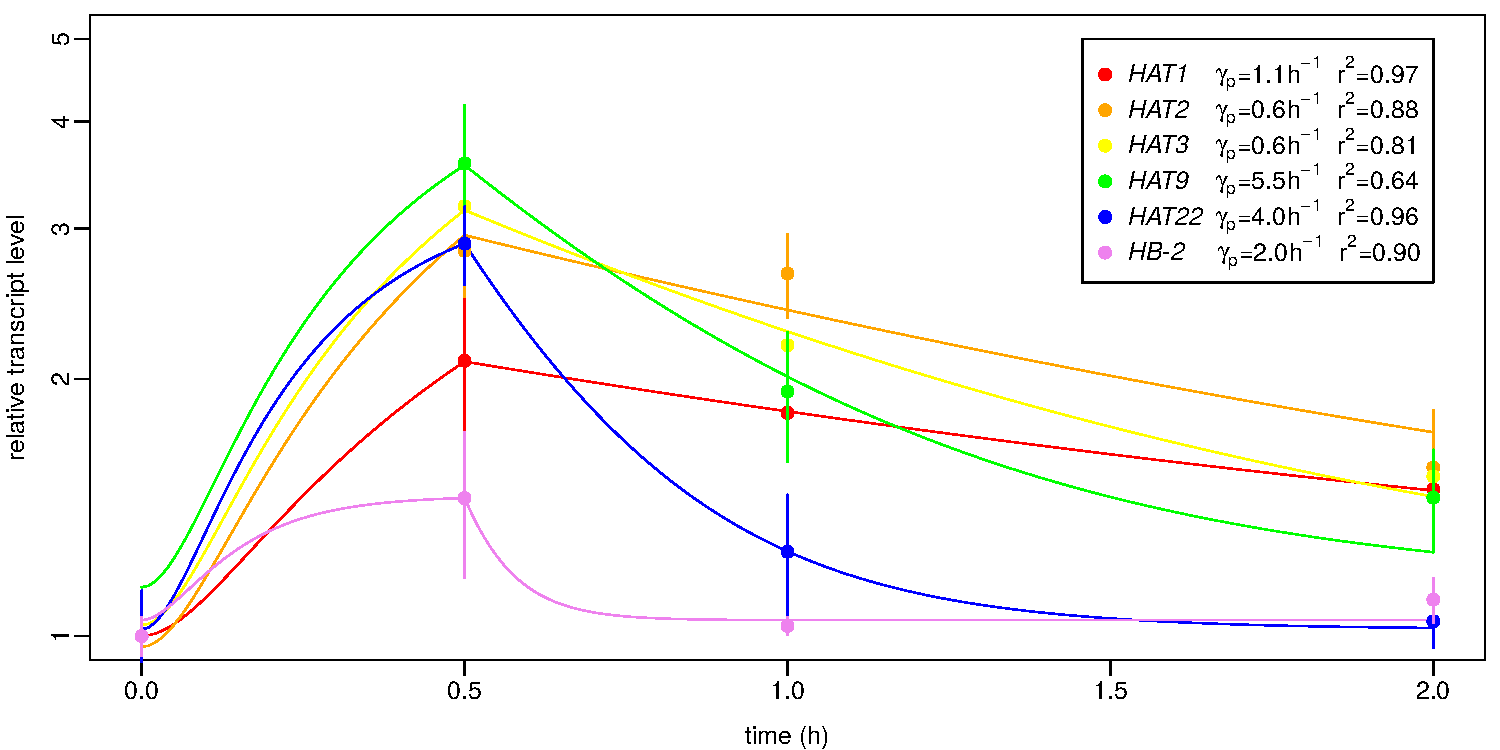
\includegraphics[width=\figwidth]{hdzip}
    \captionof{figure}{
      Many early turn-off genes are found in the HD-ZIP family, especially in the HD-ZIPII class, shown here.
    }
  \end{center}

  The rapidity of turn-off of \textit{HAT9} and \textit{HAT22} may indicate that they play a leading role in the HD-ZIPII autoregulatory network [Ohgishi. et al.].

  \subsection*{Conventional DE and model fit confidence measures are correlated}

  For microrarray/\texttt{limma} and RNA-seq/Cuffdiff DE measurements, $p$-values and FDR-adjusted $q$-values are the standard measures of confidence.
  One typically assumes that $q<0.05$ represents a 95\% probability that the measured DE is real and not a chance occurrence.
  
  In our model fits, the experimental data points, one per sample (3 reps $\times$ 4 times = 12 total),
  are individually fit, without weighting, by minimizing the variance between data and model values using the core R nonlinear minimization routine \texttt{nlm}. We then compute the standard $r^2$ coefficient
  of determination to quantify the quality of the fit.
  \begin{itemize}
  \item DE measurements are taken at a single time relative to the $t=0$ base: three independent logFC, $p$ and $q$ values result for $t=0.5$, 1 and 2 h, using six data per measurement, reusing the $t=0$ base data each time.
  \item The model fits one solution to all twelve data, and is therefore subject to variation of all, not half, of the data
  \item The model counts the $t=0$ data equally with the other data.
  \end{itemize}
  The model fit $r^2$ value, therefore, provides an independent measure of DE significance which spans the entire time course in a statistically balanced fashion.

  \begin{center}\vspace{\figtopspace}
    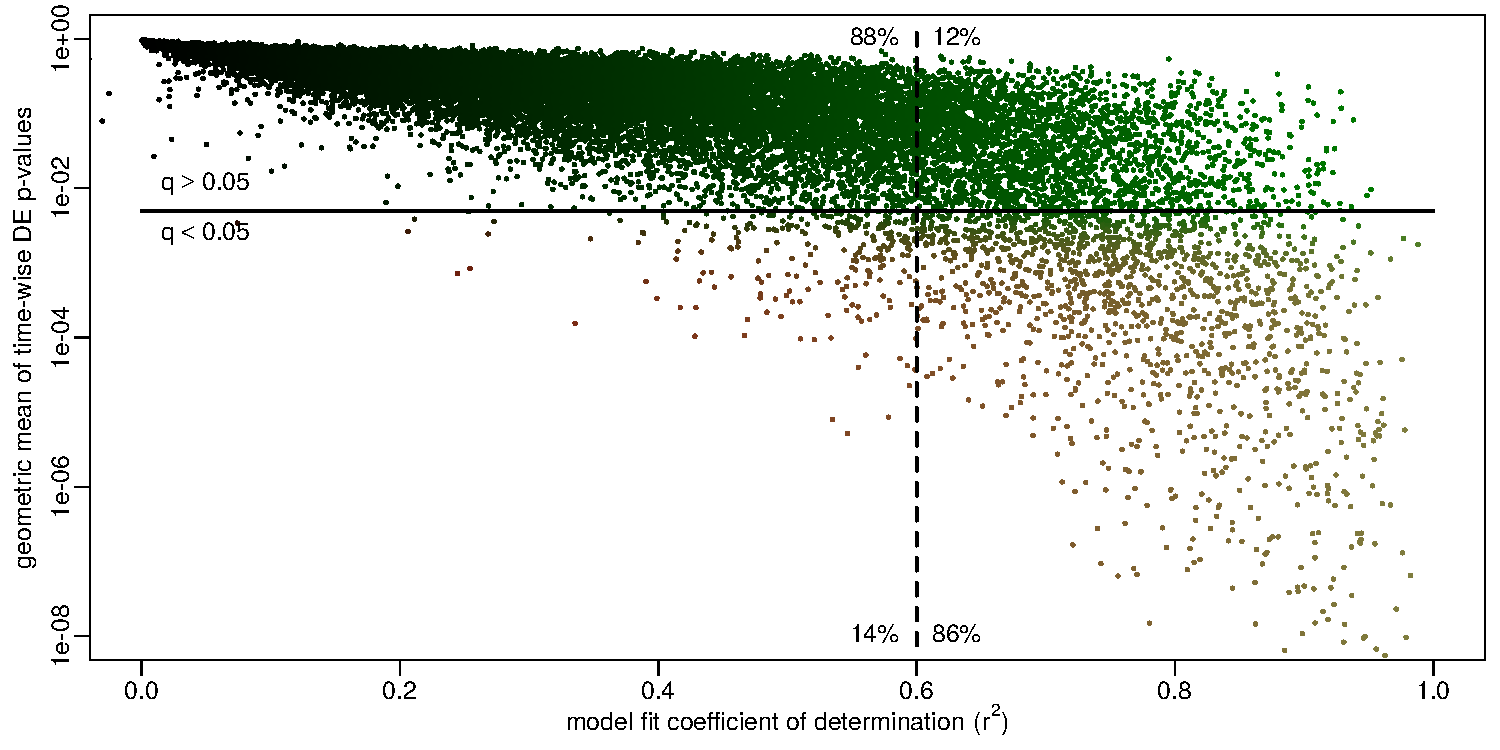
\includegraphics[width=10in,height=5in]{p-vs-r2}
    \captionof{figure}{
      Model $r^2$ values correlate with the geometric mean of the three $p$-values from \texttt{limma} DE analysis of the 22,585 GR-REV microarray transcripts which result in a model fit of any quality.
      The horizontal line shows the geometric mean of $p$-values for which $q=0.05$, representing the boundary of significant \texttt{limma}-determined DE at the $q<0.05$ level.
    }
  \end{center}

  The microarray \texttt{limma} $p$ and model-fit $r^2$ values correlate, and we have chosen $r^2>0.6$ as the significance
  level for the model fits, covering 86\% of the $q<0.05$ transcripts. A majority of significant DE time courses meet
  this model fit level in both microarray and RNA-seq series, boosting confidence in the validity of the model.

  \subsection*{Secondary targets are suggested by model fits and transcriptional response across four GR-TF lines}

  GR-REV:\textit{AHP4} rises very slowly, requiring $\gamma_p<0$ in the model, which is unphysical.
  We model the time course of \textit{AHP4} as a \textit{secondary} target with $\gamma_s>0$, and search for candidate primary targets in the four GR-TF lines which regulate it.
  If \textit{AHP4} is strictly a secondary target in the GR-TF lines in which it exhibits differential expression,
  then the corresponding primary target should also exhibit DE in those and only those lines. \textit{AHP4} is an up-regulated group L gene in GR-KAN, GR-REV and GR-STM, further suggesting that it is a secondary,
  or farther downstream target.
    
  From the RNA-seq series: 44 other genes show all up- or all down-DE in GR-KAN, GR-REV and GR-STM and none in GR-AS2.
  Of these, model fits using \textit{AHP4} as the secondary target lead to:
  \begin{itemize}
  \item 10 genes as primary targets of GR-REV with $r^2>0.6$ and $\gamma_p,\gamma_s>0$
  \item 9 genes as primary targets of GR-STM with $r^2>0.6$ and $\gamma_p,\gamma_s>0$
  \item 5 genes common to the above GR-REV and GR-STM selections
  \end{itemize}
  The RNA-seq GR-KAN:\textit{AHP4} data variance is too high to produce good model fits.

  From the microarray series, model fits to the five genes above as primaries which target \textit{AHP4} result in
  three candidates with $r^2>0.6$ and $\gamma_p,\gamma_s>0$: \textit{CRK22}, \textit{JKD} and \textit{GT2L} (At5g28300).

  %% \begin{center}
  %%   \begin{tabular}{c|ccc|ccc|ccc|ccc}
  %%     \multicolumn{1}{c}{\textbf{RNA-seq}} & \multicolumn{3}{c}{GR-AS2} & \multicolumn{3}{c}{GR-KAN}   & \multicolumn{3}{c}{GR-REV}       & \multicolumn{3}{c}{GR-STM}    \\ 
  %%     \multicolumn{1}{c}{Cuffdiff} & 0.5 & 1.0 & \multicolumn{1}{c}{2.0} & 0.5 & 1.0 & \multicolumn{1}{c}{2.0} & 0.5 & 1.0 & \multicolumn{1}{c}{2.0} & 0.5 & 1.0 & \multicolumn{1}{c}{2.0} \\
  %%     \bottomrule
  %%     \textit{CRK22} & $\times$&$\times$&$\times$ & $\times$&$\times$&-1.36 & $\times$&$\times$&-1.32 & $\times$&$\times$&-0.96   \\
  %%     \textit{JKD}   & $\times$&$\times$&$\times$ & $\times$&$\times$&-0.88 & $\times$&$\times$&-0.95 & $\times$&$\times$&-0.60   \\
  %%     \textit{GT2L}  & $\times$&$\times$&$\times$ & $\times$&$\times$&-0.70 & $\times$&$\times$&-0.79 & $\times$&-1.09&-0.97 \\
  %%     \textit{\textbf{AHP4}} & $\times$ & $\times$ & $\times$ & $\times$ & $\times$ & \textbf{0.76}  & $\times$ & \textbf{1.14} & \textbf{2.25} & $\times$ & \textbf{1.03} & \textbf{1.52} \\
  %%   \end{tabular}
  %% \end{center}
  %% \begin{center}
  %%   \begin{tabular}{c|ccc|cc|ccc}
  %%     \multicolumn{1}{c}{\textbf{microarray}} & \multicolumn{3}{c}{GR-AS2} & \multicolumn{2}{c}{GR-KAN}   & \multicolumn{3}{c}{GR-REV}    \\ 
  %%     \multicolumn{1}{c}{\texttt{limma}} & 0.5 & 1.0 & \multicolumn{1}{c}{2.0} & 0.5 & \multicolumn{1}{c}{1.0} & 0.5 & 1.0 & \multicolumn{1}{c}{2.0} \\
  %%     \bottomrule
  %%     \textit{CRK22} & $\times$ & $\times$ & $\times$ & $\times$ & -0.96 & $\times$ & $\times$ & $\times$  \\
  %%     \textit{JKD}   & $\times$ & $\times$ & $\times$ & $\times$ & -0.81 & $\times$ & $\times$ & $\times$  \\
  %%     \textit{GT2L}  & $\times$ & $\times$ & $\times$ & -0.73 & -0.85    & $\times$ & $\times$ & $\times$  \\
  %%     \textit{\textbf{AHP4}} & $\times$ & $\times$ & $\times$  & $\times$ & $\times$ & $\times$ & \textbf{1.01} & \textbf{2.06} \\
  %%   \end{tabular}
  %%   \captionof{table}{
  %%     logFC values for three putative targets of \textit{KAN}, \textit{REV} and \textit{STM} which target \textit{AHP4}.
  %%   }
  %% \end{center}

  \begin{center}\vspace{\figtopspace}
    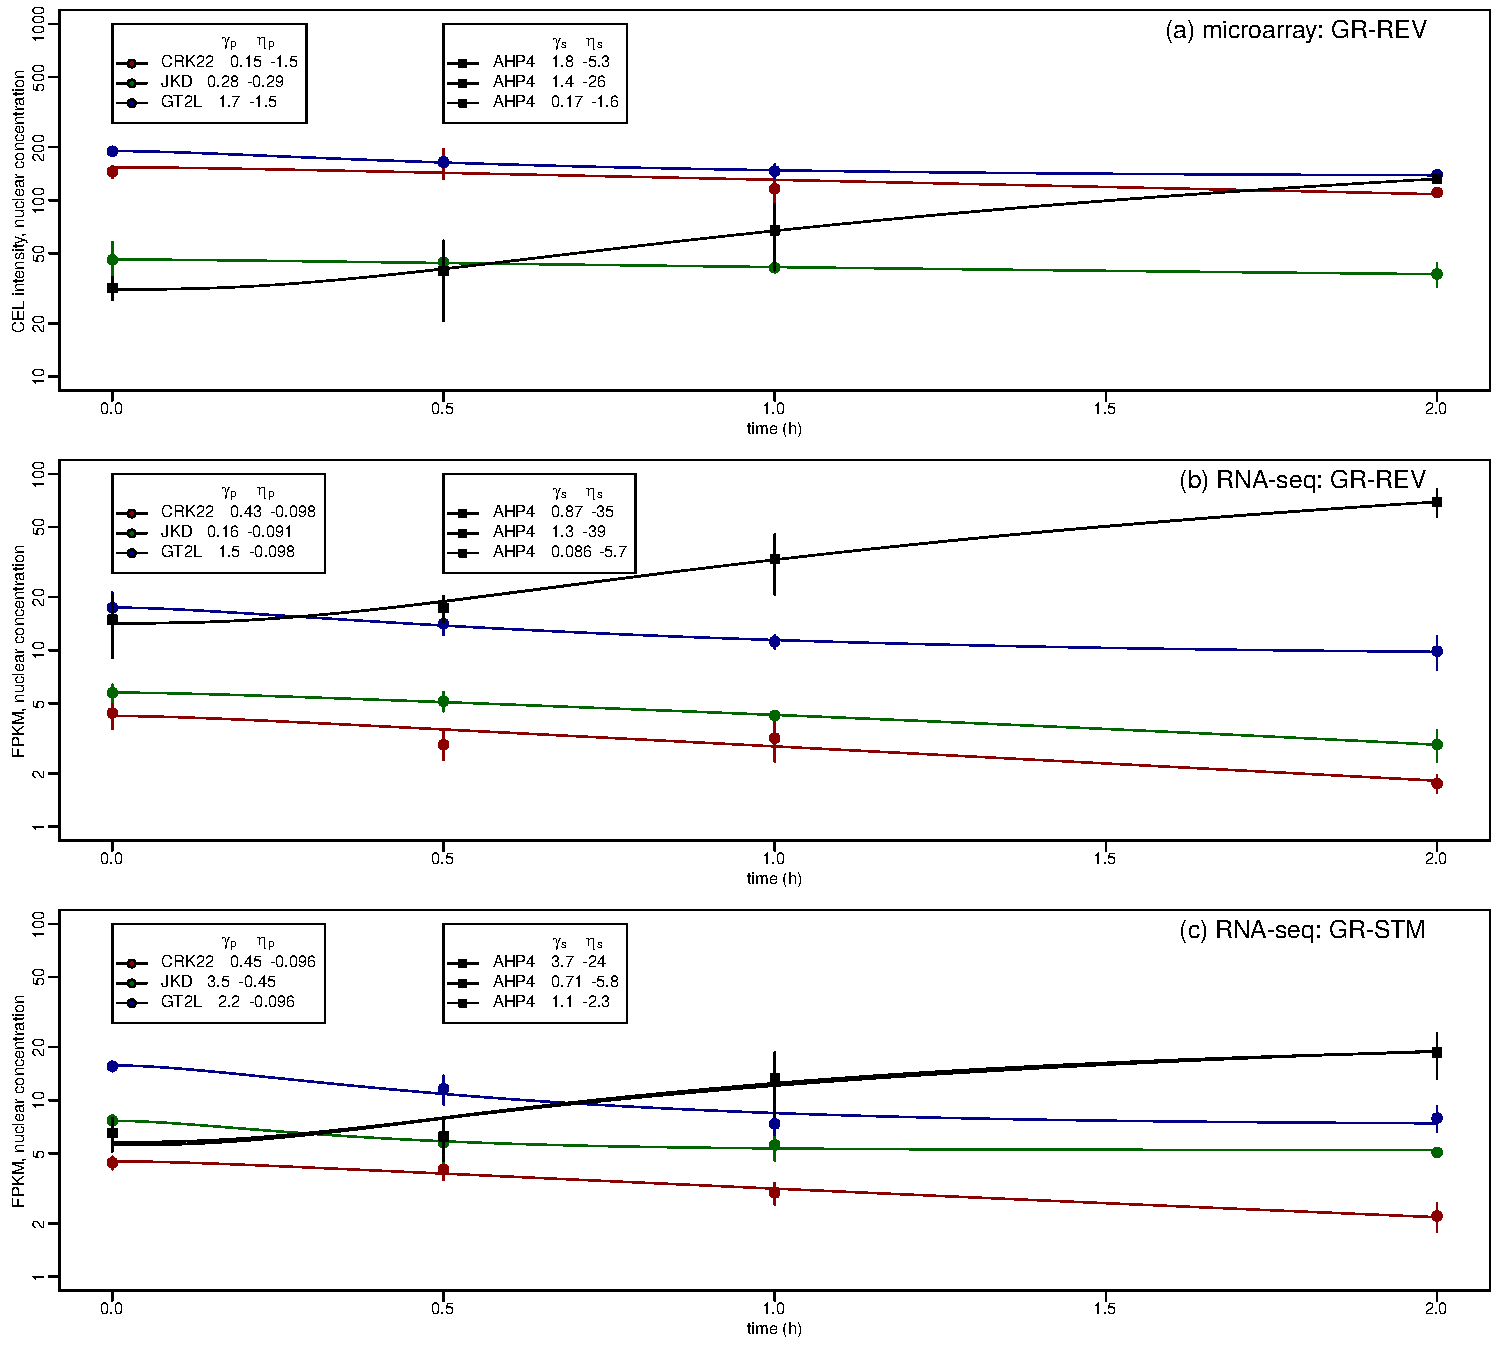
\includegraphics[width=\figwidth]{AHP4}
    \captionof{figure}{
      Three genes are well simulated as down-regulated targets of \textit{KAN}, \textit{REV} and \textit{STM}, which in turn down-regulate \textit{AHP4}.
    }
  \end{center}

  We regard these three genes as candidate primary targets of \textit{KAN}, \textit{REV} and \textit{STM}, which, in turn, target \textit{AHP4}.
  (One of these three, \textit{GT2L}, is a member of the Trihelix TF family, but \textit{AHP4} has not been reported as a target.)
  Also note that the three candidate primary targets are \textit{down}-regulated in GR-KAN, GR-REV and GR-STM lines.
  This suggests that they \textit{repress} \textit{AHP4}, which then overexpresses its mRNA as their expression is reduced by the induced TF.
  
  %----------------------------------------------------------------------------------------
  %	CONCLUSIONS
  %----------------------------------------------------------------------------------------

  \section*{CONCLUSIONS}
  \color{CarnegiePriBlue}

  \begin{enumerate}
  \item DEX-induced GR-TF transcription time courses can be modeled with a set of linear ODEs with parameters ($\gamma_p$,$\eta_p$) describing the
    primary target response and ($\gamma_s$,$\eta_s$) describing the secondary target response.
  \item Model fits use data in a balanced fashion, rather than the overemphasis of $t=0$ data in time-wise DE measurements.
  \item Model-determined metrics $\kappa$ and ${\rm logFC}_\infty$ characterize the primary target response in a time-independent manner, as opposed to
    misleading single-time DE measurements.
  \item The model simulates transcription turn-off by setting $\eta_p$ or $\eta_s$ to 0 at an appropriate time, matching autoregulated genes in the HD-ZIPII family.
  \item The model simulates primary and secondary transcriptional responses, supporting target discovery and inference of gene regulatory networks.
  \end{enumerate}

  \color{Black}

  %----------------------------------------------------------------------------------------
  %	FORTHCOMING RESEARCH
  %----------------------------------------------------------------------------------------

  \section*{Forthcoming Research}

  \begin{enumerate}
  \item Improve model to make robust fits for ``black box'' analysis, perhaps in a Web application, with data and fit diagnostics
  \item Measure tighter time course of selected GR-TFs and targets using qPCR
  \item Measure GR-TF nuclear import and mRNA accumulation using flourescent probes
  \item Measure mRNA induction in real time with CRISPRi activation?
  \end{enumerate}

  %----------------------------------------------------------------------------------------
  %	REFERENCES
  %----------------------------------------------------------------------------------------

  \nocite{*} % Print all references regardless of whether they were cited in the poster or not
  \bibliographystyle{plain} % Plain referencing style
  \bibliography{hokin-aspb2017} % Use hokin-aspb2017.bbl - regenerate with bibtex

  %----------------------------------------------------------------------------------------
  %	ACKNOWLEDGEMENTS
  %----------------------------------------------------------------------------------------

  \section*{Acknowledgements}
  
  \noindent This research was funded by National Science Foundation grant \#0929413.

  
\end{multicols}
\end{document}
